\chapter{Künstliche Intelligenz}
\thispagestyle{fancy}
\section{Definition: künstliche Intelligenz}
Um den Begriff der künstlichen Intelligenz besser verstehen zu können, soll zunächst allgemein festgehalten werden, was Intelligenz bedeutet. Obwohl die Intelligenz ein abstraktes, gesellschaftliches Konstrukt ist, lässt sie sich wie folgt definieren:

\begin{quote}
\glqq  Intelligenz ist die Fähigkeit, aus Erfahrung zu lernen, Probleme zu lösen und das Wissen zur Anpassung an neue Situationen einzusetzen.\grqq{} \parencite[S. 400]{psychologie}
\end{quote}

Das Ziel mit einer künstlichen Intelligenz soll nun also sein, dass ein Computer diese Fähigkeit erlernt. Somit lässt sich künstliche Intelligenz als Teilgebiet der Informatik definieren, welches sich mit der Erforschung von Mechanismen des intelligenten menschlichen Verhaltens befasst. Dies geschieht durch Simulation mithilfe künstlicher Artefakte. Diese Artefakte sind für gewöhnlich Programme auf einem Computer \parencite[]{wichert}. Nach \citet[23]{russell2012knstliche} lässt sich dieses Teilgebiet weiter in vier Kategorien aufteilen:\\

\begin{enumerate}
    \item \textbf{Menschliches Denken}
    \item[] Der Computer soll in der Lage sein zu denken. Dabei soll er die Fähigkeit haben, Entscheidungen treffen zu können, Probleme zu lösen und sich eigenständig neues Wissen aneignen.
    
    \item \textbf{Menschliches Handeln}
    \item[] Mit den Fähigkeiten des menschlichen Denkens soll es dem Computer möglich sein, diese Dinge aktiv umsetzen zu können. Er handelt aktiv, nachdem er eine Entscheidung getroffen hat oder versucht aktiv ein Problem zu lösen.
    
    \item \textbf{Rationales Denken}
    \item[] Der Computer soll ein allgemeines, logisches Denken erlernen können, das auf mathematischen Formalismen basiert. Dies geschieht mittels programmiertechnischer Modelle und befähigt ihn zu logisch zu schließen und zu agieren.
    
    \item \textbf{Rationales Handeln}
    \item[] Er werden sogenannte \textit{rationale Agenten erzeugt}, also technische Operatoren, die aktiv handeln können. Sie haben das Ziel, immer das beste Ergebnis zu erzielen \parencite[S. 25]{russell2012knstliche}.
\end{enumerate}


Es sollen also Systeme entstehen, die so denken und agieren wie Menschen und ebenso rational denken und agieren wie sie. Dafür werden rationale Agenten geschaffen, die aus diesen Eigenschaften hervorgehen und entsprechend handeln.

\section{Ebenen der künstlichen Intelligenz}
Auch innerhalb der künstlichen Intelligenz lassen sich verschiedene Ebenen ausmachen, etwa die Begriffe des \textit{Machine Learnings} oder \textit{Deep Learnings}. \citet[]{copeland_2021} erklärt, dass die beiden Begriffe aus der Entwicklung der künstlichen Intelligenz entstanden seien, denn Deep Learing sei eine weitere Ebene, welche sich innerhalb von Machine Learning entwickelte (Abbildung \ref{KIKreise}). Obwohl die Konzepte des Deep Learnings genauso alt sind, wie die des Machine Learnings, sei es erst seit wenigen Jahren möglich, sie in großem Maße einzusetzen. Der Autor hält fest, dass die zu dem Zeitpunkt benötigte Computerleistung, wie etwa schnelle GPUs, damals nicht existierte. Der größte Unterschied zwischen Machine und Deep Learning seien die sogenannten \textit{neuronalen Netze} des Deep Learnings.\\

\begin{figure}[ht]
    \centering
    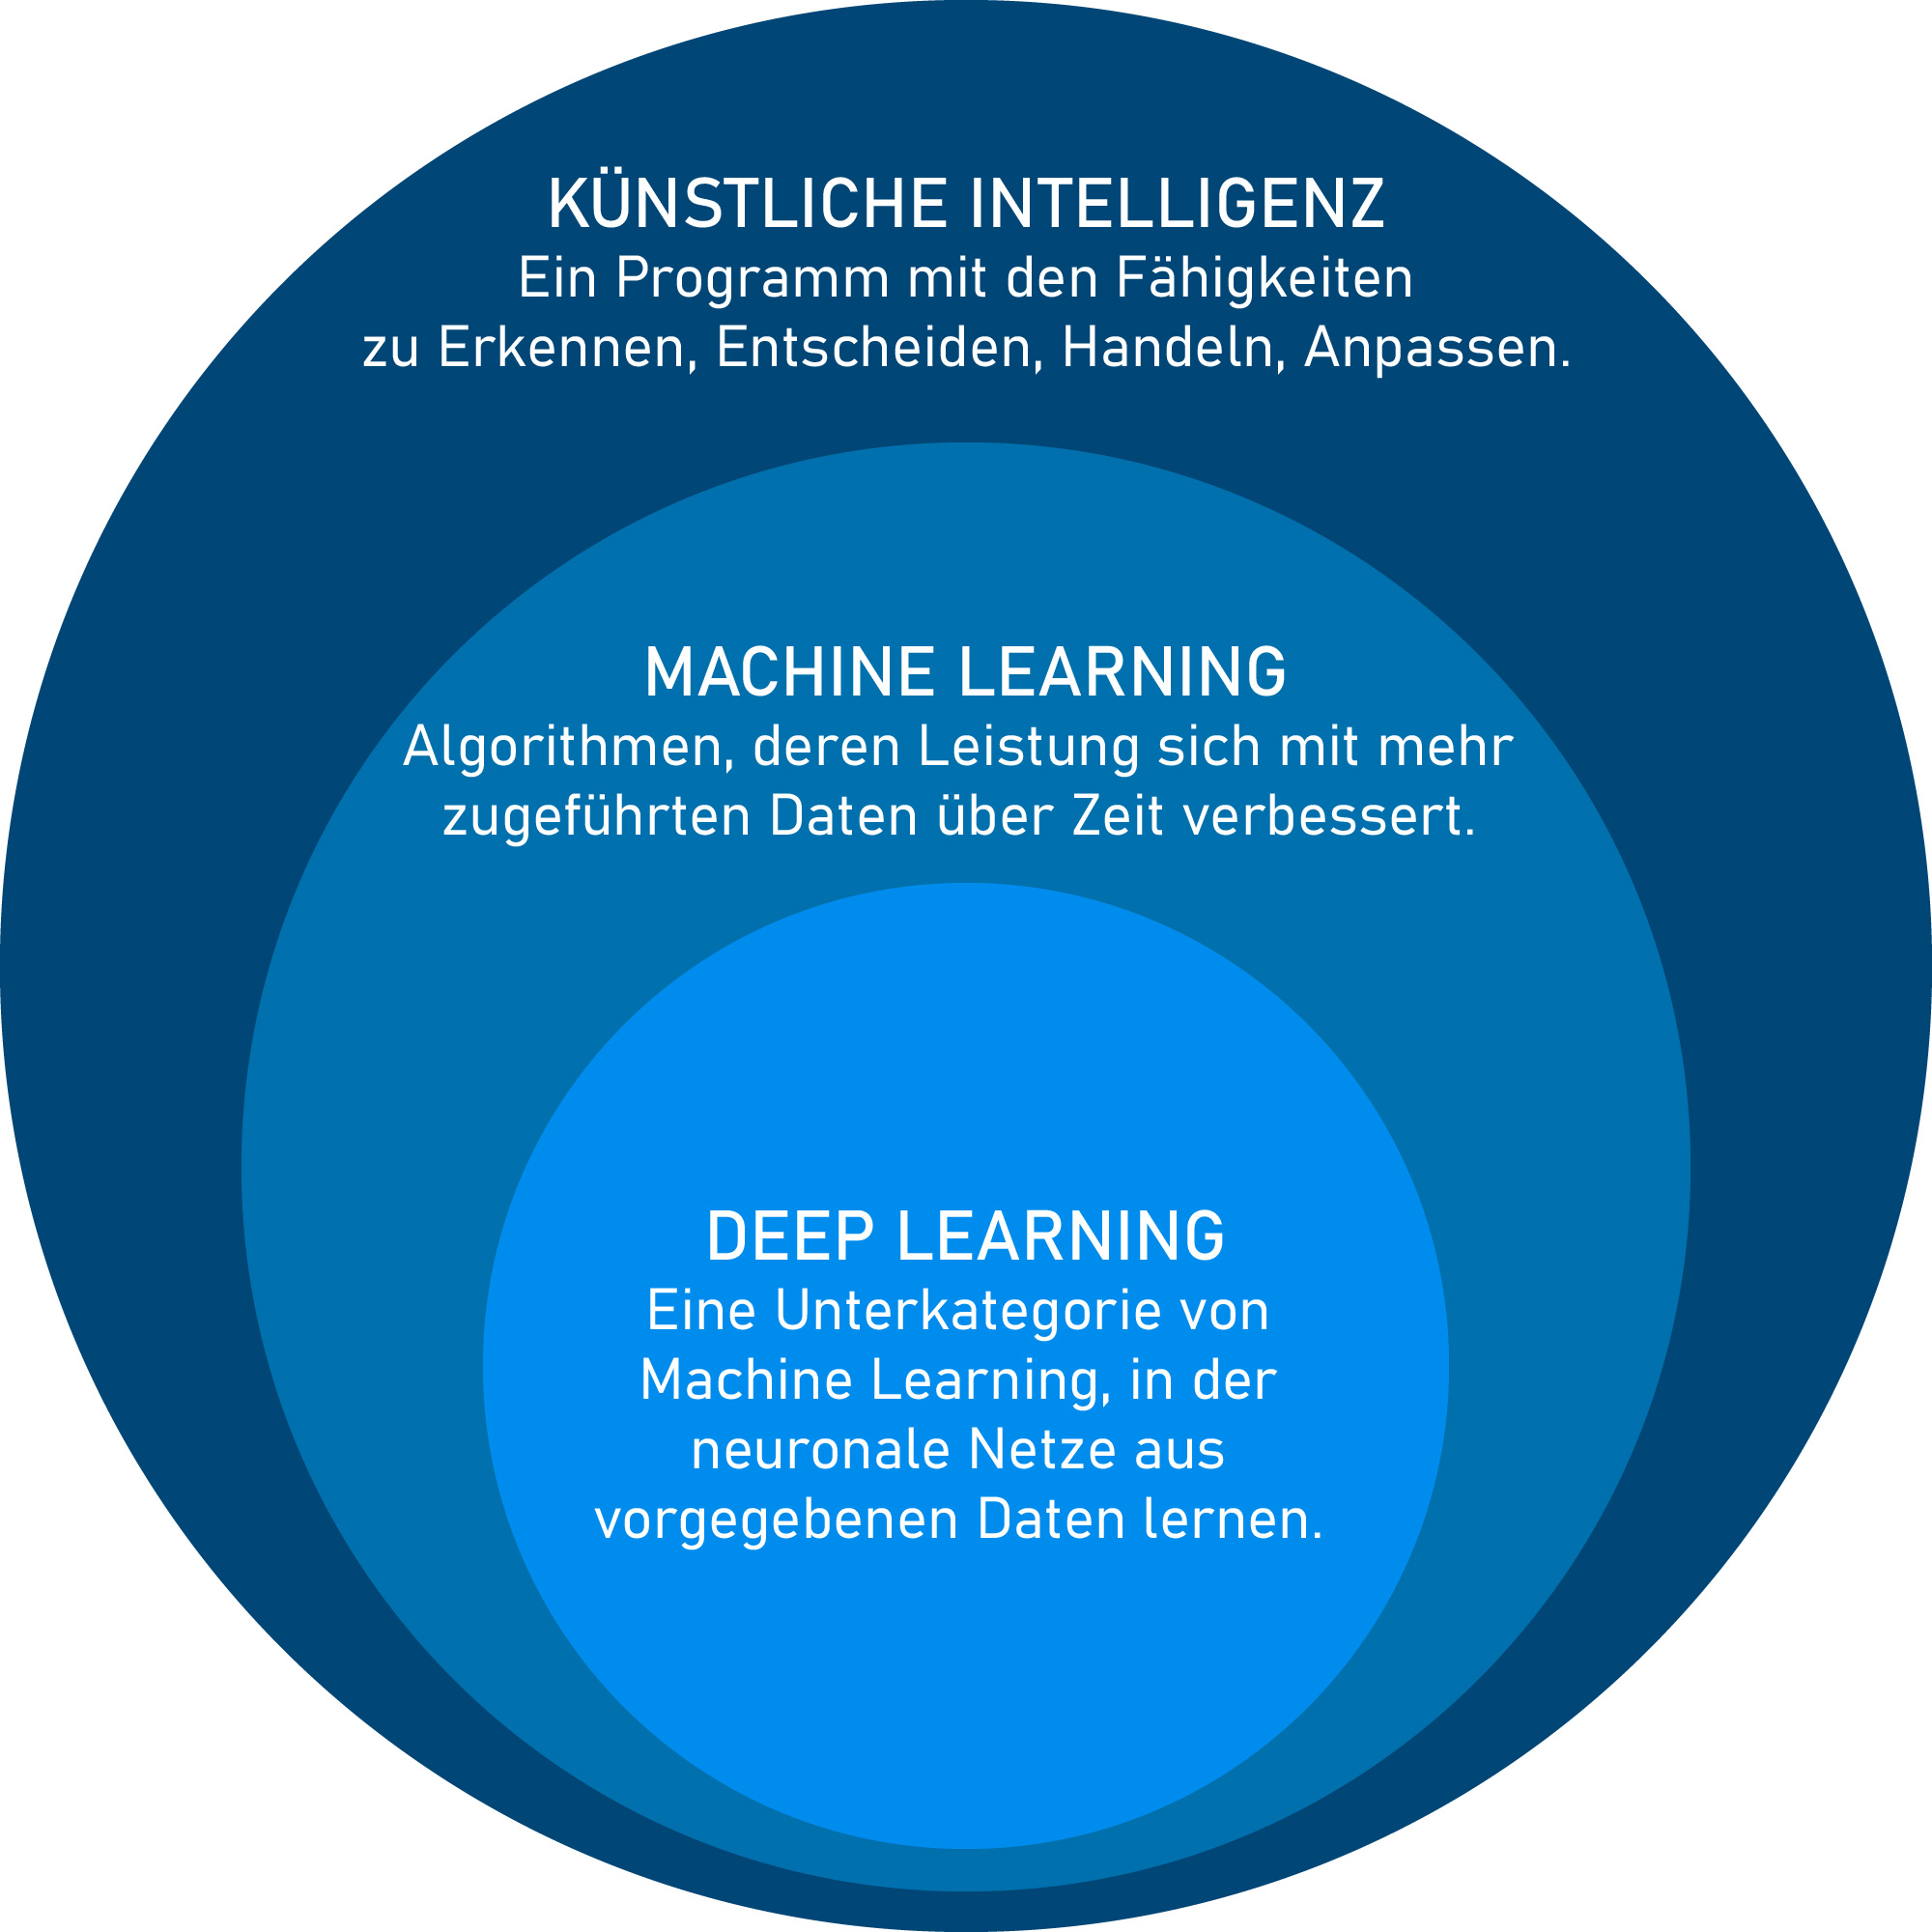
\includegraphics[width=8cm]{bilder/KIKreise2.jpg}
    \caption{Ebenen der künstlichen Intelligenz.}
    \source{Philipp Benner in Anlehnung an \citet[]{wuttke_2022}.}
    \label{KIKreise}
\end{figure}

\citet[]{Janiesch.2021} erklären, dass Machine Learning vom Menschen vorgegebene Merkmale nutze, um einem Algorithmus beizubringen, welche Elemente in den vorliegenden Daten eine hohe Relevanz haben und das Ergebnis beeinflussen würden. Erhält der Algorithmus Daten, so könne dieser mithilfe der Merkmale über eine gewisse Zeit hinweg selbstständig lernen und seine Funktion verbessern. Dieses Definieren der Merkmale nannten die Autoren \textit{Feature Engineering}. Soll zum Beispiel festgestellt werden, wie hilfreich eine Bewertung in einem Online-Shop ist, ließe sich als Merkmal die Wortwahl, oder die Anzahl der Wörter nehmen. \\

Ebenso wird nach \citet[]{Janiesch.2021} kein Feature Engineering beim Deep Learning verwendet. Dort hingegen kommen neuronale Netze zum Einsatz, die wie im menschlichen Gehirn auf vielen miteinander verbundenen Neuronen basieren. Die Neuronen lernen selbstständig, welche Merkmale ein positives oder negatives Ergebnis verursachen. Somit bietet der Einsatz von Deep Learning Netzen einen Zeitvorteil und es ist möglich, dass die Netze Merkmale erlernen, die ein Mensch während des Feature Engineerings nicht beachtet hat. Die genaue Arbeitsweise von neuronalen Netzen folgt im nächsten Abschnitt.\\

Mittlerweile sind die Konzepte des Deep Learnings ein essenzieller Forschungsbereich innerhalb künstlicher Intelligenzen. Das zeigt beispielsweise, dass das meist zitierte Whitepaper in der Kategorie \textit{Computer Vision and Pattern Recognition} im Jahr 2020, eines aus der Forschung an Deep Learning Netzwerken ist. Mit dem Titel \textit{Deep Residual Learning for Image Recognition}, publiziert durch ein Forscherteam bei Microsoft \parencite[]{crew2020}, wurde dargelegt, wie mit speziellen neuronalen Ebenen in einem Deep Learning Netzwerk das Lernverhalten des Netzes verbessert werden könnte.


\section{Einführung in neuronale Netze}
Im weiteren Verlauf dieser Arbeit sollen tiefergehende Einblicke in Deep Learning und neuronale Netzen gegeben werden. Dazu wird primär die Literatur des Autors \textit{Tariq Rashid} verwendet. Er ist ein qualifizierter Datenanalyst und publizierte einige Bücher über neuronale Netze und Algorithmen \parencite[]{educative-no-date}. Außerdem besitzt er einen Master of Science in Künstlicher Intelligenz sowie einen weiteren Master in Naturwissenschaften \parencite[]{linkedin-no-date}.\\

\citet[S. 32]{traiq_neuron} erklärt, dass Deep Learning versuche, sich die Funktionsweise des menschlichen Gehirns zunutze zu machen, indem einzelne Neuronen erschaffen, ein elektrisches Eingangssignal übernehmen und ein anderes Signal ausgeben würden, so zu sehen in Abbildung \ref{neuronen2}.


\begin{figure}[ht]
    \centering
    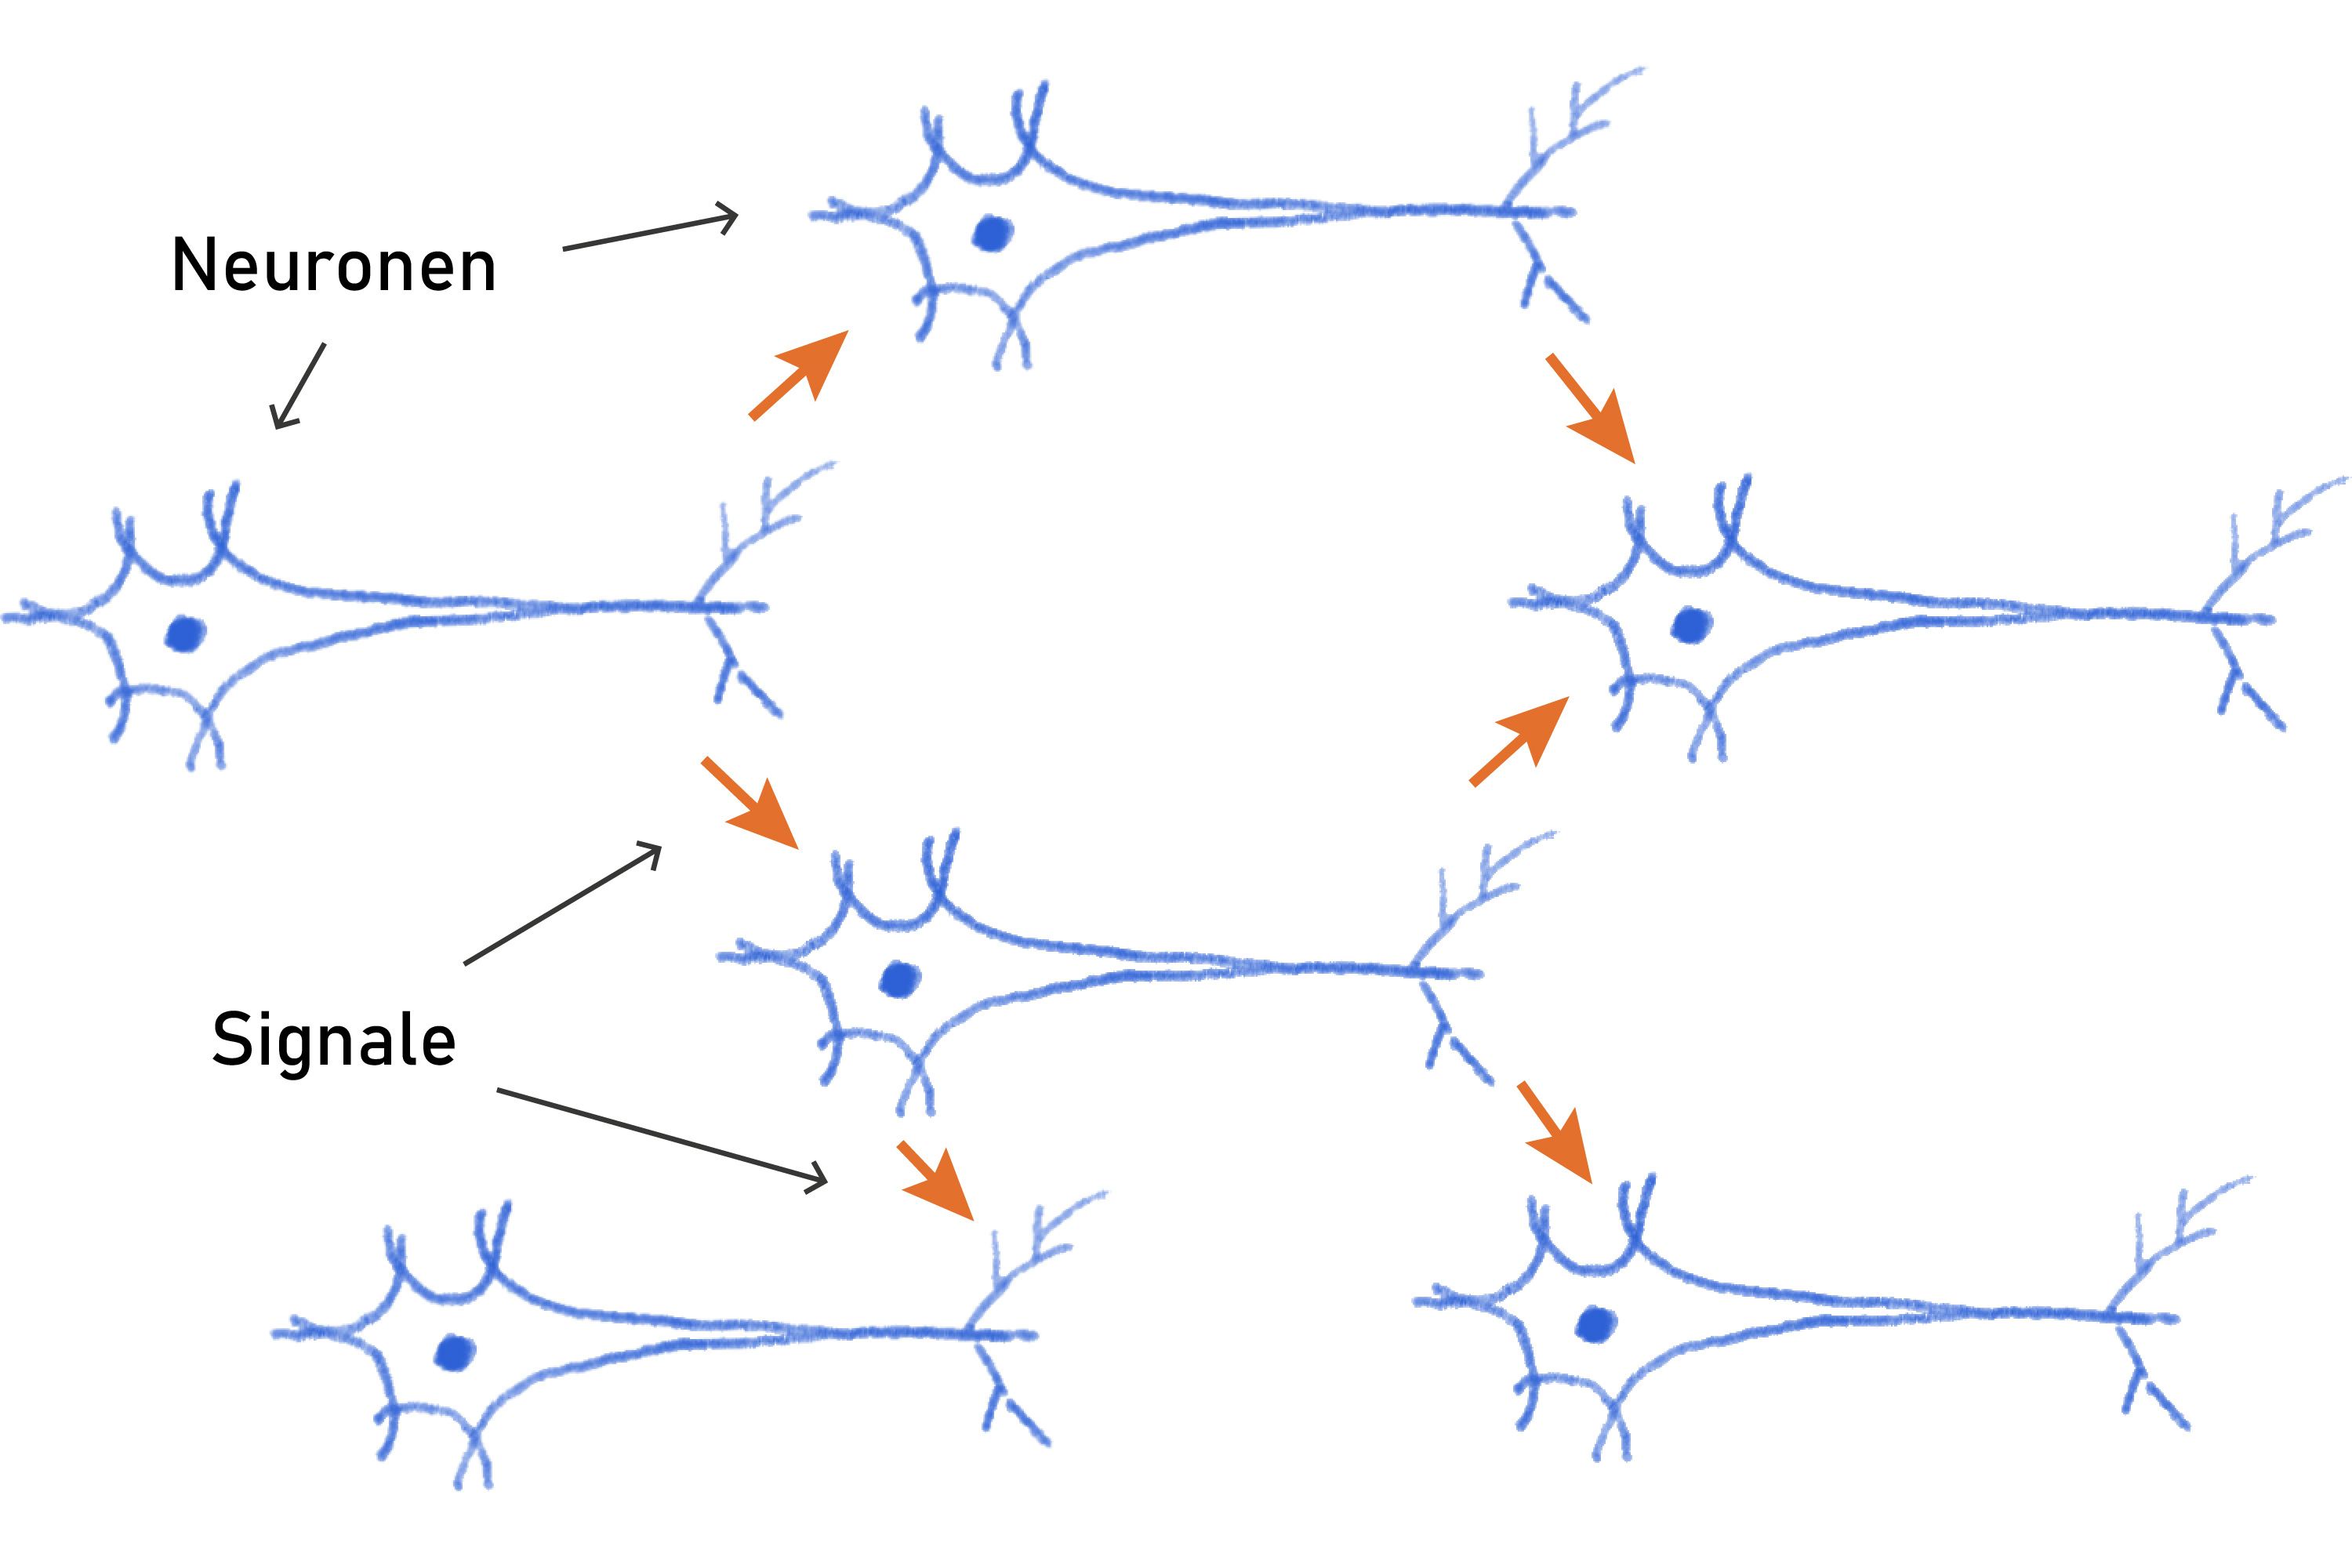
\includegraphics[width=10cm]{bilder/NeuronenGehirn.jpg}
    \caption{Darstellung eines neuronalen Netzes im menschlichen Gehirn.}
    \source{Philipp Benner in Anlehnung an \citet[36]{traiq_neuron}}
    \label{neuronen2}
\end{figure}

 Der Autor führt fort, dass die Eingangssignale jedoch nicht direkt wieder ausgegeben würden, sondern einen gewissen Schwellenwert überschreiten müssten, bevor eine Ausgabe erzeugt werden würde. Im Gehirn findet sich eine Vielzahl solcher Neuronen, deren Ein- und Ausgänge miteinander verbunden seien. So ist ein Neuron beispielsweise mit drei weiteren Neuronen in seinen Eingängen verbunden und erzeugt erst ein Ausgabesignal, wenn mindestens zwei der drei Eingänge ein elektrisches Signal erhalten. Dieses Konzept lässt sich ebenso digital abbilden und ist der Grundstein für künstliche neuronale Netze. Im Folgenden soll die Bezeichnung \textit{neuronales Netz} für das künstliche, digitale Netz in einem Computerprogramm stehen.\\

\section{Aufbau und Funktion neuronaler Netze}

Wie hilft ein solches Netz nun, menschliches Denken zu imitieren? Im Folgenden soll die Arbeitsweise eines neuronalen Netzes an einem vereinfachten Beispiel erklärt werden. Das neuronale Netz soll anhand eines Graustufenbildes erkennen, ob ein Hund auf einem Bild zu finden ist. Ein Ausgangswert zwischen 0,0 und 1,0 soll anzeigen, wie sicher sich das Netz ist, einen Hund erkannt zu haben. 0,0 bedeutet kein Hund, 1,0 bedeutet, das Netz ist sich sicher, einen Hund erkannt zu haben. Um das Netz zu verstehen, werden im Folgenden Begriffe zum Verständnis der Abbildung \ref{neuronalesnetz} erklärt.\\

\begin{figure}[ht]
    \centering
    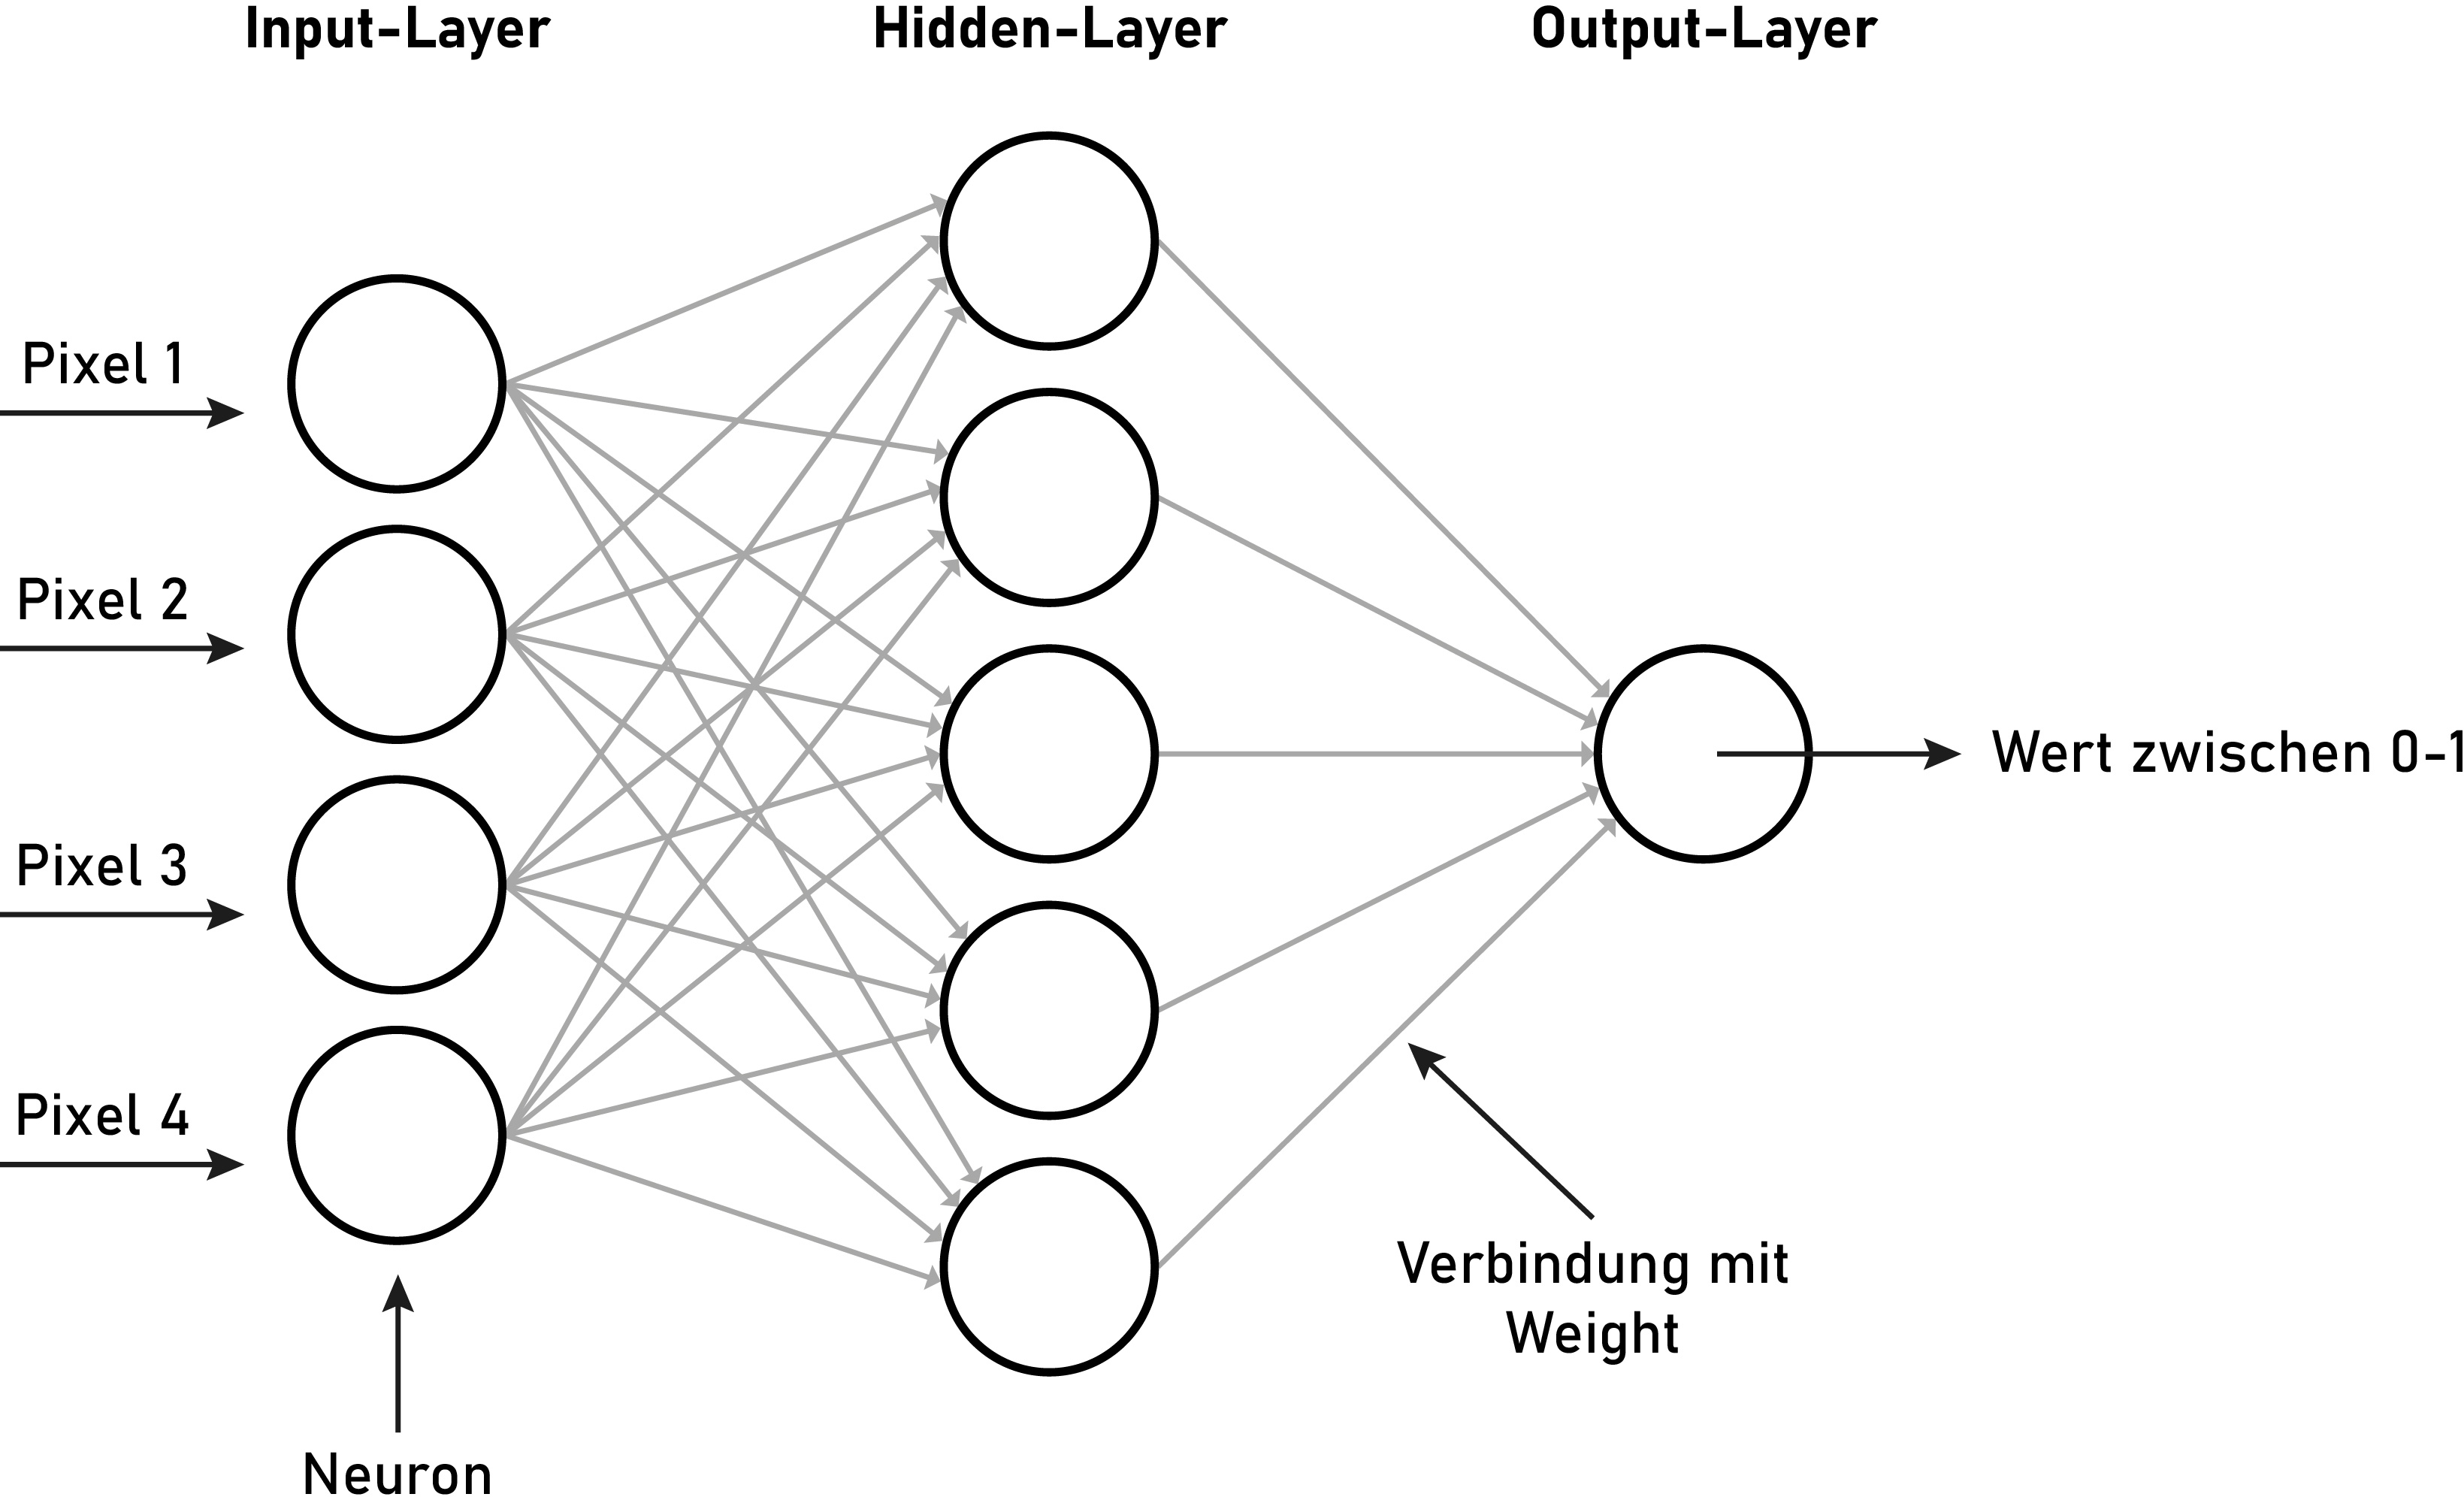
\includegraphics[width=11cm]{bilder/kuentlNetz.jpg}
    \caption{Darstellung eines künstlichen neuronalen Netzes.}
    \source{Philipp Benner}
    \label{neuronalesnetz}
\end{figure}

\subsubsection*{Neuron} Ein Neuron stellt einen Knotenpunkt im Netz dar. Es ist mit weiteren Neuronen durch seine Ein- und Ausgänge verbunden. Durch die Verbindungen fließen nun aber keine elektrischen Signale, sondern Zahlen. Am Ende einer jeden Verbindung steht ein Zahlenwert, der mit allen weiteren Verbindungen, die an einem Neuron anliegen, summiert und in die \textit{Activation Function} eingesetzt wird. Diese Funktion erzeugt einen einzelnen Ausgangswert pro Neuron, welcher wiederum über die Verbindungen an andere Neuronen weitergegeben wird \parencite[S. 40]{traiq_neuron}.

\subsubsection*{Activation Function} Zu Deutsch \textit{Aktivierungsfunktion}. Abbildung \ref{stufenfunktion} zeigt eine Stufenfunktion innerhalb eines Neurons. Alle Zahlenwerte am Eingang des Neurons werden summiert und müssen einen bestimmten Schwellenwert überschreiten. Erst dann wird der Ausgabewert von 0,8 erzeugt. Weitere Aktivierungsfunktionen sind zum Beispiel die nach \citet{Hahnloser2000} bei positiven Werten linear ansteigende \textit{ReLU} Funktion, bei der das Ausgabesignal denselben Wert hat wie das Eingabesignal, wenn das Eingabesignal größer als Null ist. Die S-Artige Sigmoidfunktion sei eine weitere wichtige Aktivierungsfunktion laut \citet[S. 34]{traiq_neuron}. Sie sei einfach zu berechnen und unterdrücke zu niedrige Eingangssignale.

\begin{figure}[ht]
    \centering
    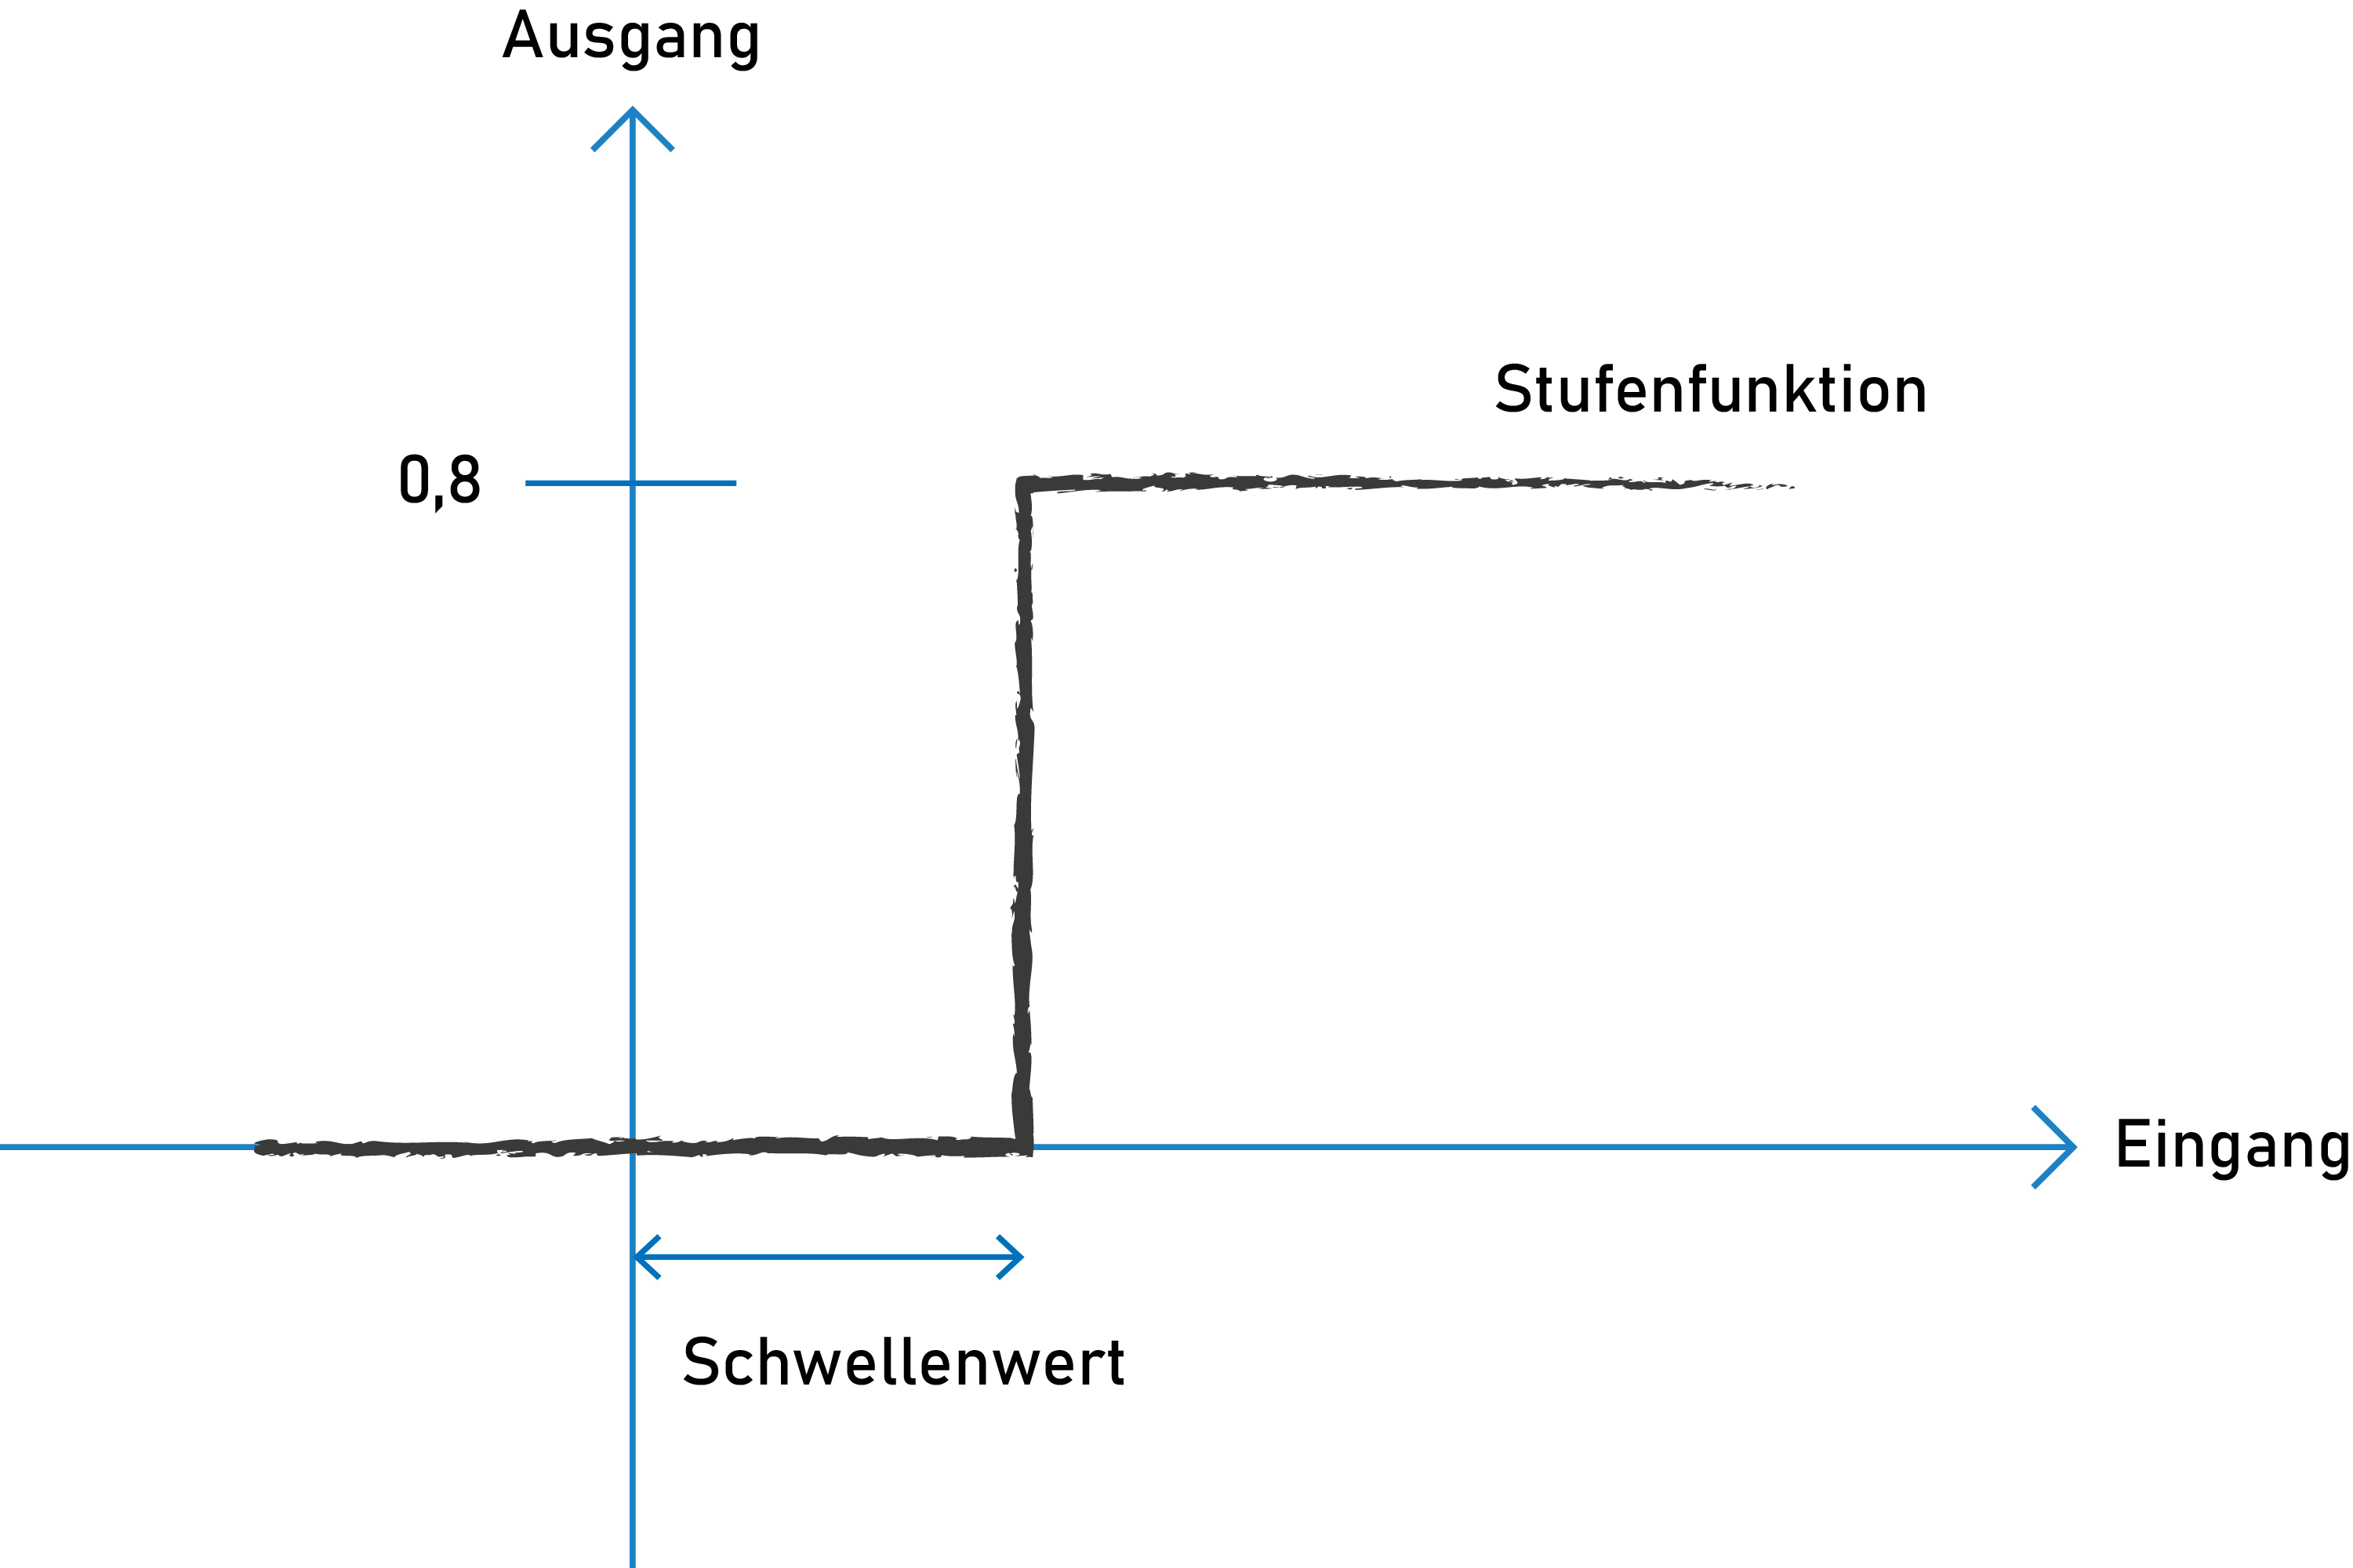
\includegraphics[width=9cm]{bilder/Stufenfunktion.jpg}
    \caption{Aktivierung eines Neurons mittels der Stufenfunktion.}
    \source{Philipp Benner in Anlehnung an \citet[33]{traiq_neuron}}
    \label{stufenfunktion}
\end{figure}

\subsubsection*{Weight} \citet[37]{traiq_neuron} erklärt, dass die uns bekannten Verbindungen zwischen den Neuronen einem sogenannten \textit{Weight} oder Gewicht unterliegen würden. Dies ist ein einfacher Multiplikator für den Ausgangswert eines Neurons. Beträgt etwa der Ausgangswert nach der Aktivierungsfunktion 0,8 und das Gewicht 0,5, so beläuft sich der neue Ausgangswert, der am Eingang des nächsten Neurons anliegt, auf 0,4.

\subsubsection*{Input Layer} Wie in Abbildung \ref{neuronalesnetz} zu sehen, besteht das Netz aus drei vertikalen Ebenen oder Layern. Der Input Layer stellt hierbei die erste Ebene dar. Um dem Netzwerk ein Bild zeigen zu können, werden aus den Pixeln des Bildes Input-Neuronen erzeugt, die jeweils den Helligkeitswert des Pixels annehmen. Beträgt die Auflösung des Bildes etwa 100 $\cdot$ 100 Pixel, so entstehen 10.000 Input-Neuronen. In \ref{neuronalesnetz} werden zur besseren Übersicht nur vier der 10.000 Input-Neuronen dargestellt. Alle Neuronen werden anschließend mit allen anderen Neuronen im darauffolgenden Hidden Layer verbunden. Auf die Eingabewerte wird keine Aktivierungsfunktion angewendet \parencite[S. 41]{traiq_neuron}.

\subsubsection*{Hidden Layer} Dieser stellt den zweiten Layer im Netz dar und enthält eine vom Programmierer vordefinierte Anzahl an Neuronen, die mit dem Input Layer verbunden sind. \citet[]{ramsundar-no-date} erklären, dass Layer, deren Neuronen mit allen Neuronen aus dem vorhergehenden Layer verbunden seien, die Bezeichnung \textit{Fully-connected-Layer} hätten. Es kann einen oder mehrere Hidden Layer geben, mit einer verschiedenen Anzahl an Neuronen \parencite[S. 52]{traiq_neuron}.

\subsubsection*{Output Layer} Dieser Layer stellt die Ausgabe des Netzes dar. Im Beispiel der Abbildung \ref{neuronalesnetz} laufen die Verbindungen des Hidden Layers in einem einzelnen Neuron im Output Layer zusammen und erzeugen eine letzte Ausgabe. Diese Ausgabe stellt die Sicherheit des Netzes als Wert von 0,0 bis 1,0 dar. Ein Output Layer kann aber auch mehr als nur ein Neuron haben. Mehr Neuronen als im Input Layer sind ebenso möglich \parencite[]{kukreja2016introduction}. \citet[36]{traiq_neuron} bezeichnet ein fertig aufgebautes Netz mit all seinen Layern und Funktionen als \textit{(engl.) Model}.


\section{Training eines neuronalen Netzes}
Im Folgenden wird das Training eines neuronalen Netzes vereinfacht erläutert. Damit das Netz nun lernt, die Bilder richtig zu klassifizieren, werden diesem verschiedene Bilder mit und ohne Hund gezeigt. Dazu wird ein ausgewogener Datensatz von Bildern mit und ohne Hund erstellt. Die Bilder erhalten ebenso ein Label mit \textit{0}, wenn kein Hund zu sehen ist, und mit \textit{1}, wenn das Bild einen Hund enthält. Anschließend, so führt der Autor fort, werde der Datensatz in \textit{Trainingsdaten} und \textit{Testdaten} unterteilt. Trainingsdaten werden zum Trainieren des Netzes verwendet, wohingegen die Testdaten erst nach dem Training zum Einsatz kommen. Somit lässt sich das Netz mit Daten testen, welches es noch nie zuvor gesehen hat, um genauere Aussagen über dessen Effizienz treffen zu können.\\

Laut \citet[302]{GoodBengCour16} würden den Gewichten des Netzes zufällige Werte aus einer Gauß-Verteilung zugewiesen werden, um ein effizientes Lernen zu ermöglichen. Mehrere Hidden Layer, die mit identischen Gewichten initialisiert werden, würden stets dasselbe lernen und somit könne sich das Netz nicht weiterentwickeln. Aber wie genau lernt nun ein neuronales Netz?\\

\citet[136]{traiq_neuron} erklärt, dass die Pixel der einzelnen Bilder in Input-Neuronen umzuwandeln seien, und die Helligkeitswerte dieser Pixel durch das Netz geschleust werden sollen. \citet[S. 42]{traiq_neuron} beschreibt, dass für jede Verbindung eines Neurons dessen Ausgabewert mit dem Gewicht der Verbindung multipliziert werde. Dieses Ergebnis pro Verbindung wird mit den anliegenden Verbindungen am Eingang eines Neurons summiert und in die Aktivierungsfunktion eingesetzt. Der neue Ausgabewert wird erneut mit dem Gewicht pro Verbindung multipliziert und der Kreislauf beginnt von vorn für den nächsten Layer im Netz. \citet[S. 44]{traiq_neuron} zufolge, würden komplexe Matrixmultiplikationen durchgeführt, um alle Verbindungen an allen Neuronen zu berechnen. Am Ende entsteht ein einziger Ausgangswert im Output Layer. Nun wird der Ausgangswert mit dem Label des Bildes verglichen. Falls das Bild eines Hundes am Netz angelegt wurde, sollte der Ausgangswert im besten Fall 1,0 betragen. Zu Beginn des Trainings wird das nicht der Fall sein, da das Netz noch nicht ausreichend lernen konnte. Nun muss der Fehlerwert, oder englisch \textit{Loss}, berechnen werden, den das Netz erzeugt hat.\\

Beispielsweise erzeugt das Netz für das Hundebild den Ausgabewert 0,3. Somit beträgt der Fehlerwert 0,7. Jetzt startet die sogenannte \textit{Backpropagation} oder etwa \textit{Fehlerrückführung}. \citet[S. 59]{traiq_neuron} erklärt, dass sie dazu genutzt werde, die Gewichte im Netzwerk zu verfeinern, um eine immer bessere Ausgabe mit geringerem Fehlerwert zu erzeugen. Anschließend beginne die Rückführung von hinten im Netz und es werde der Fehlerwert proportional zum Gewicht einer Verbindung aufgeteilt. Bei diesem Prozess werde der Fehlerwert kleiner, je weiter der Fehler zum Anfang des Netzes aufgeteilt werde. Anschließend wird jedes Gewicht so aktualisiert, sollte dasselbe Bild wieder durch das Netz geschleust werden, würde der Fehler geringer sein. \citet[21]{traiq_neuron} zufolge, sollen sich die Gewichte nur in geringem Maße verfeinern, da jedes Bild einen anderen Fehlerwert erzeuge. Dieses Maß würde über die sogenannte \textit{Learning Rate} geregelt. Die Verfeinerung der Gewichte und die Berechnung von komplexeren Fehlerwerten ist die Aufgabe des sogenannten \textit{Optimizers}, einem Algorithmus, der anhand einer mathematischen Funktion, das Minimum des Fehlerwertes für alle Gewichte im Netz sucht und es dahin gehend optimiert \parencite[]{doshi-2019}. Laut \citet[]{bushaev-2018} sei im Jahr 2014 ein Optimizer namens \textit{ADAM} veröffentlicht worden, der speziell für den Einsatz in Deep Neural Networks entworfen wurde. Ein Vorteil von ADAM sei, dass dieser adaptive Learning Rates benutze und somit individuelle Werte für die einzelnen Gewichte ermitteln konnte. Dies steigere die Performance des neuronalen Netzes. \\

Nach \citet[]{brownlee-2019} lasse sich das Training mit sogenannten \textit{Batches} verfeinern. Dabei werden nicht nach jedem Bild, welches durch das Netz geschleust wurde, die Gewichte aktualisiert, sondern erst nach einer gewissen Anzahl von Bildern. Mehrere Bilder seien Teil eines Batches, dessen Größe über die \textit{Batch Size} geregelt werde. Eine Batch Size von zehn enthält also zehn Bilder. Bei insgesamt 100 Bildern gibt es somit 10 Batches. Erst nachdem alle Bilder durch das Netz geschleust wurden und ein Fehlerwert für jedes Bild berechnet wurde, werden die Gewichte aktualisiert.\\

Nun wird dem Netz jeder Batch mit den dazugehörigen Labeln gezeigt, der Fehler berechnet und die Gewichte entsprechend aktualisiert. In der Praxis wiederholt sich dieser Durchlauf mehrmals in sogenannten Epochen. Bei zehn Epochen würde das Netz alle Bilder zehnmal sehen, was dem Optimizer erlaubt, die Effizienz des Netzes zu steigern \parencite[155]{traiq_neuron}.\\

Dies ist ein kleiner Teil an Mechanismen, die beim Training eines neuronalen Netzes ablaufen. Eine genauere Erläuterung passt jedoch nicht in den Rahmen dieser Arbeit. Daher soll ein Einblick in eine Art neuronaler Netze folgen, die auch als Teil dieser Forschung verwendet werden.

\section{Convolutional Neural Networks}
Sobald ein künstliches neuronales Netz für die Bildverarbeitung eingesetzt wird, bietet es sich an, anstatt Fully-connected-Layer mithilfe von \textit{Convolutional Layer} ein sogenanntes \textit{Convolutional-neural-Network} (CNN) zu schaffen. In diesen speziellen Layern wird ein Bild nicht mehr in eine Vielzahl an Neuronen zerlegt, sondern erhält seine ursprüngliche Form. \citet[135]{tariq_gan} erläutert, wenn das Bild das Netz durchlaufe, werde es mit einem Filter, dem sogenannten \textit{Kernel}, Pixel für Pixel gescannt. In Abbildung \ref{CNN} ist ein zweidimensionales Input Array zu sehen, das die Werte eines Pixelbildes darstellt. Dem Autor zufolge werde ein Kernel der Größe 3 $\cdot$ 3 erstellt und schrittweise über das Bild geschoben. Dabei würden die Werte im Input Array mit den Werten des Kernels multipliziert und anschließend alle entstehenden Produkte summiert werden. Dadurch entstehe ein Output Array einer geringeren Pixelanzahl mit den gefilterten Werten. Der Autor bezeichnet den Prozess des Verschiebens und das daraus resultierende Output Array als \textit{Faltung}.

\begin{figure}[ht]
    \centering
    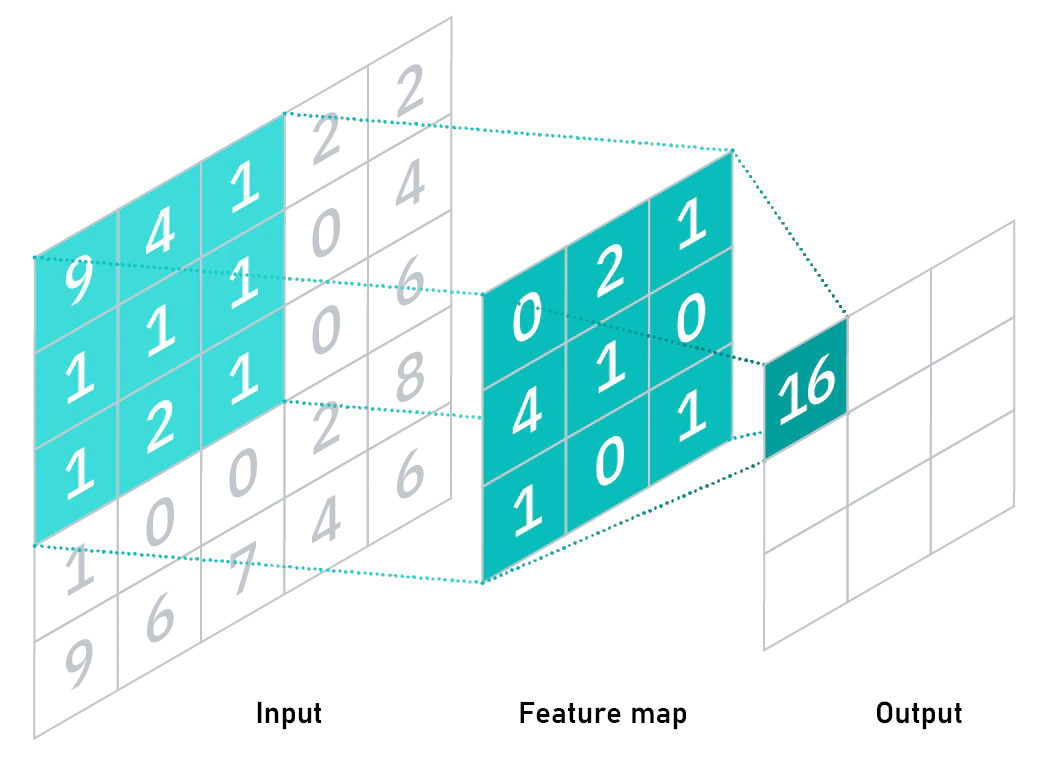
\includegraphics[width=9cm]{bilder/cnn.jpg}
    \caption{Arbeitsweise eines Convolutional Layer.}
    \source{Philipp Benner in Anlehnung an \citet{ibm-cloud-education-2021}}
    \label{CNN}
\end{figure}


\citet[133]{tariq_gan} zufolge werden die Werte im Kernel beim Training des Netzes verfeinert, damit eine sogenannte \textit{Feature Map} für bestimmte Merkmale im Bild entstehe. Diese Feature Maps seien laut \citet[]{brownlee-2019} auch die \textit{Channels} mit dem ein CNN arbeite. Ein RGB Bild habe für seine drei Farbkanäle die gleiche Anzahl an Input Channels im CNN. In den weiteren Convolutional Layern lassen sich die Größen für die Feature Maps/Channels aber nach Belieben erhöhen. Eine Feature Map lernt zum Beispiel, ob eine gewisse Pixelanordnung im Bild, etwa eine Linie oder ein Kreis zu sehen ist. Durch Kombination mehrerer Convolutional Layer lassen sich Merkmale auf einer höheren Ebene wie ein Auge oder eine Nase herausarbeiten. CNNs erreichen damit eine höhere Effizienz als herkömmliche Fully-connected-neural-Networks und benötigen weniger Speicher innerhalb der GPU \parencite[154]{tariq_gan}.

\section{Resiudal Neural Networks}
Je mehr Convolutional Layer ein neuronales Netz hat, desto wahrscheinlicher sei es laut \citet[]{nandepu-2021}, dass dieses Netz an den sogenannten \textit{Vanishing Gradients} leide. Dieses Phänomen handle von Layern am Anfang eines Netzes, die sich während des Trainings nicht mehr optimieren ließen, da der Fehler, der zu diesen Layern zurückgeführt würde, immer kleiner werde und irgendwann bei Null läge. Dann verschlechtere sich die Performance eines KI-Modells drastisch. Der Autor führt fort, dass sogenannte \textit{Residual Neural Networks} (RNN) eine Lösung für dieses Problem bieten würden. Dabei würden Abkürzungen in das Netz eingebaut werden, um den Weg der Backpropagation zu verkürzen. In Abbildung \ref{resnet} ist die schematische Darstellung eines sogenannten \textit{Residual Blocks} zu sehen. Der Autor erklärt, dass die eingehenden Daten durch zwei Verbindungen fließen würden. Diese würden durch die obere und untere Verbindung in Abbildung \ref{resnet} dargestellt. Die Blöcke der unteren Verbindung bestehen aus einem Convolutional Layer gefolgt von einem sogenannten \textit{Batch Normalization Layer} der die Input-Daten des Netzes neu berechnet und sie so formt, dass der Wertedurchschnitt der Daten bei null und die Varianz bei eins liegt \parencite[]{batchnorm}. \citet[]{nandepu-2021} führt fort, dass der Output des Batch Normalization Layers wird anschließend in die ReLU-Aktivierungsfunktion eingesetzt würde. Dieser Convolutional-Block wiederhole sich bis auf die Aktivierungsfunktion zweimal. Die Daten der oberen Verbindung würden ebenfalls durch einen Convolutional und Batch Normalization Layer fließen, jedoch komme hierbei nur ein einzelner Block zum Einsatz. Diese Verbindung werde auch als Abkürzung oder \textit{Shortcut} bezeichnet, da sie einige Layer überspringt. Am Ende des Residual Blocks würden die Daten aufsummiert werden und anschließend in den nächsten Layer im Netz fließen.

\begin{figure}[ht]
    \centering
    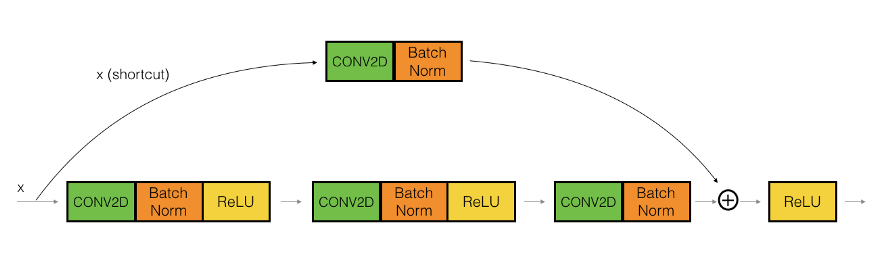
\includegraphics[width=14cm]{bilder/resnet.png}
    \caption{Aufbau eines Residual Blocks.}
    \source{\citet[]{iprathore-2020}}
    \label{resnet}
\end{figure}

Da die Daten, die durch das Netz fließen über die Shortcuts einen geringeren Weg zum ersten Layer während der Backpropagation haben, lassen sich Vanishing Gradients reduzieren und die Performance des KI-Modells aufrechterhalten.

\section{Generative Adversarial Networks}
Neuronale Netze werden nicht nur zur Klassifizierung eingesetzt, sondern sind auch in der Lage, neue Inhalte selbstständig zu erschaffen. \citet{Goodfellowgan} erforschten für diese Zwecke die sogenannten \textit{Generative Adversarial Networks} (GAN) oder \textit{Generativ gegnerische Netzwerke}. Gegnerisch deshalb, da bei diesem Konzept zwei künstliche Netzwerke gegeneinander antreten. Abbildung \ref{GAN} zeigt den Aufbau eines GANs, das handschriftliche Ziffern erzeugen soll. Ein Netzwerk ist ein sogenannter \textit{Diskriminator}, dieser entscheidet, ob sein Input echt oder künstlichen Ursprungs ist. Der Gegenspieler ist der \textit{Generator}, der Inhalte künstlich erzeugen kann. Schritt für Schritt versucht er seine Ergebnisse zu verbessern, um den Diskriminator später täuschen zu können, sodass die eigentlich künstlichen Ergebnisse als echt eingestuft werden.

\begin{figure}[ht]
    \centering
    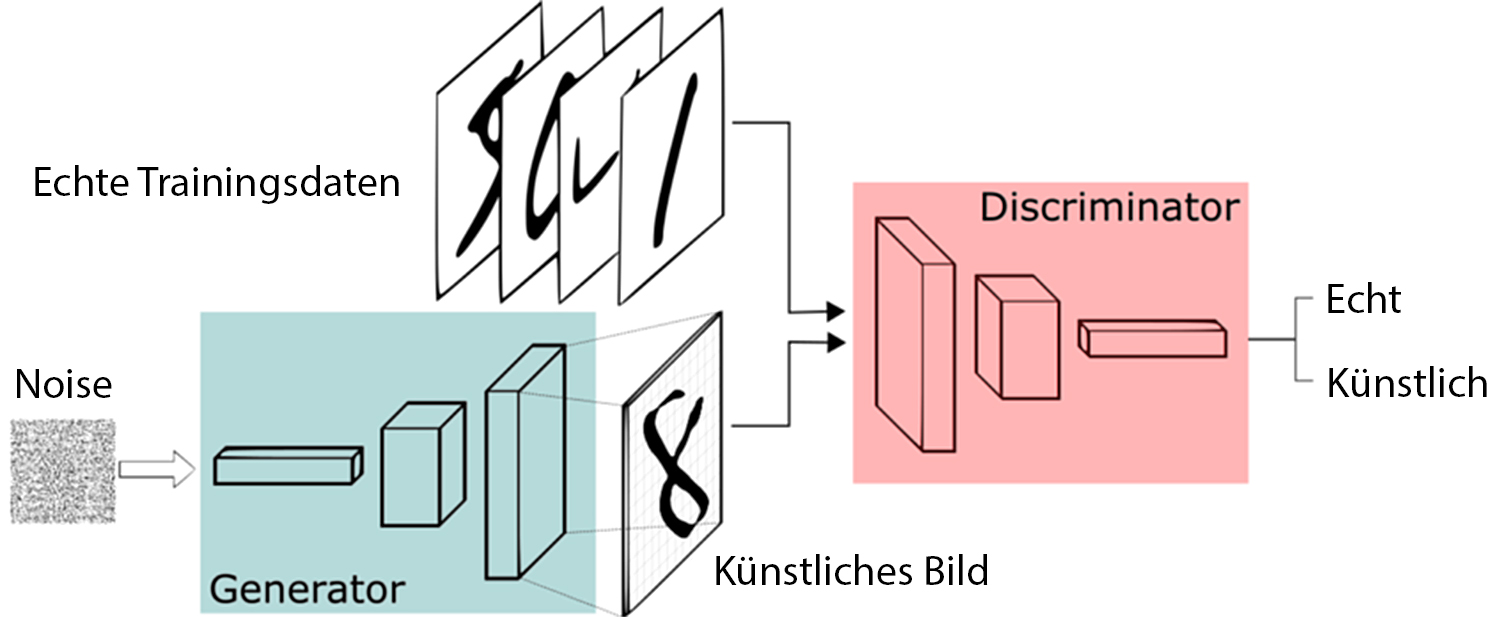
\includegraphics[width=11cm]{bilder/GAN_Net.jpg}
    \caption{Aufbau eines Generative Adversarial Networks.}
    \source{Philipp Benner in Anlehnung an \citet{silva-2020}}
    \label{GAN}
\end{figure}

Solche Netzwerke werden häufig für die Herstellung von statischen oder Bewegtbildern eingesetzt. Aber auch die Erstellung von 3D-Objekten oder Nutzung in Chatbots ist möglich \parencite[]{luber-2021}.

\section{Aufbau und Training eines Generative Adversarial Networks}
Generative Adversarial Networks, die zur Bildverarbeitung eingesetzt werden, basieren oftmals auf Convolutional Neural Networks um künstliche Bilder erzeugen. Im vorhergehenden Abschnitt wurden CNNs genutzt, um aus einem zweidimensionalen Pixelbild einen einzigen Ausgabewert zu erzeugen. Dafür wurden die Dimensionen und deren enthaltenen Werte schrittweise reduziert. \citet[61]{tariq_gan} erläutert, dass dieses Prinzip bei der Verwendung von GANs umgekehrt werde. Es ist möglich aus einer geringen Anzahl an ein- oder zweidimensionalen Werten, hochauflösende, mehrdimensionale Daten zu erschaffen. In Abbildung \ref{GAN} wird etwa ein zweidimensionales Pixelbild mit zufällig gewählten Werten, sogenanntes \textit{Noise}, an den Input des Generators angelegt. Das Bild hat die Auflösung 10 $\cdot$ 10 Pixel. Um die Auflösung des Bildes zu erweitern und den Noise in erkennbare Zahlen zu wandeln, kommen spezielle, umgekehrte Convolutional Layer zum Einsatz. \citet[145]{tariq_gan} erklärt, dass diese Erweiterung mit einer \textit{Transposed Convolution} oder \textit{transponierten Faltung} stattfinde. Dabei würden zusätzliche Pixel zwischen den bereits vorhandenen eingefügt, um ein größeres Bild zu erhalten. In Abbildung \ref{GAN} ist eine schematische Darstellung zu sehen, in der drei Transposed Convolutional Layer innerhalb des Generators die Auflösung eines Bildes erhöhen. 
Der Diskriminator nutzt hingegen normale Convolutional Layer, um Daten zu reduzieren und das Bild mit 0,0 für künstliche Bilder und 1,0 für echte Bilder zu klassifizieren. \\

Die Trainingsschleife wird im Folgenden nach \citet[65\psq]{tariq_gan} beschrieben. Im ersten Schritt wird dem Diskriminator ein echtes Trainingsbeispiel gezeigt und mitgeteilt, dass die Klassifizierung 1,0 betragen soll. Daraufhin wird dieser basierend auf dem Fehlerwert aktualisiert. Im zweiten Schritt wird dem Diskriminator eine künstliche Ausgabe des Generators gezeigt und mitgeteilt, dass die Klassifizierung 0,0 sei. Danach wird diese ebenfalls aktualisiert. Der Autor führt fort, dass im dritten Schritt dem Diskriminator erneut die Ausgabe des Generators gezeigt wird, diesmal wird aber dem Generator mitgeteilt, dass die Klassifizierung 1,0 betragen soll. Nun wird also nicht mehr der Diskriminator, sondern der Generator mit dem Fehlerwert aktualisiert und lernt somit, sich zu verbessern. Beide Netze sind zu Beginn schlecht im Generieren und Klassifizieren. Beide stehen im Wettbewerb gegeneinander und versuchen nach jeder Aktualisierung etwas besser zu werden. Im besten Fall hat der Generator nach genügend Trainingsepochen gelernt, visuell fehlerfreie, handschriftliche Ziffern zu erzeugen, die selbst von einem Menschen nicht mehr unterschieden werden können.

\section{Probleme und Fehlerquellen}
Es reicht nicht aus, einen Datensatz durch ein funktionierendes neuronales Netz zu schleusen und ein perfektes Ergebnis zu erwarten. Selbst nach etlichen Epochen und Tagen an Training kann es sein, dass ein Netz keine ausreichenden Ergebnisse liefert. Deshalb müssen neuronale Netze laufend auf verschiedene Arten optimiert werden. Im Folgenden sollen ein paar Probleme und Fehlerquellen erläutert werden.\\

\subsubsection*{Hardware Limitierung}
Laut \citet[]{fevbre-no-date} ließen sich Neuronale Netze schneller und effektiver auf einer GPU anstatt auf dem Prozessor trainieren. Dabei gäbe es die Limitierung, dass das Modell mit seinen Parametern vollständig in den Speicher der GPU passen müsse. Für kleine Modelle stelle dies kein Problem dar. Werden jedoch viele komplexe Ebenen wie Convolutional Layer hinzugefügt, würde die Speichergrenze schnell erreicht werden. Dieses Problem trat zum Beispiel während des Trainings des für diese Arbeit angefertigten Modells auf. Eine Möglichkeit ist es, die Layer im Modell zu reduzieren, was jedoch die Lernfähigkeit beeinträchtigt. Alternativ lassen sich die Modelle auf mehreren Grafikkarten parallel trainieren \parencite[]{giacaglia-2021}.

\subsubsection*{Black Box}
\citet[]{dickson-2019} erklärt, dass ein künstliches Neuronales Netz ein komplexes Geflecht aus selbst erlernten Parametern sei und es ließe sich schwierig vorhersagen, wie das Netz auf bestimmte Eingaben reagiere. Für triviale Aufgaben sei dies kein Problem, da solche Modelle jedoch zum Beispiel in medizinischen Diagnosen eingesetzt würden, sei eine hohe Zuverlässigkeit des Modells gefordert.

\subsubsection*{Unausgewogener Datensatz}
Die Qualität der Ausgabe eines Netzes hängt unter anderem sehr von den Daten ab, die dem Netz gezeigt werden. Dabei gilt es besonders darauf zu achten, diese Daten sorgfältig auszuwählen, damit der Datensatz keiner Verzerrung, dem sogenannten \textit{Bias} unterliegt. Als Beispiel sollten dem Diskriminator eines GANs während dem Training zur Zahlenerkennung, auch möglichst alle Zahlen gleichermaßen gezeigt werden. Würden ihm viele Zweier, aber nur wenig Neuner gezeigt werden, so könnte er diese nur schlecht erkennen \parencite[]{hao-2020}. Ebenso spielt die Qualität der Daten eine wichtige Rolle. Wird ein neuronales Netz zur Objekterkennung auf Bildern trainiert, sollten die Trainingsdaten beispielsweise nicht Abgeschnitten, verrauscht oder verschwommen sein \parencite[]{prov-international-inc-2022}.

\subsubsection*{Fehlende Balance}
\citet[67]{tariq_gan} zufolge sollen sich die im Wettbewerb gegeneinander stehenden Netze eines GANs stets in gleichem Maße verbessern. Eile der Diskriminator etwa dem Generator voraus, so schaffe es dieser nicht mehr aufzuholen. Sollte der Diskriminator zu langsam lernen, so verbessere der Generator seinen Output nicht und erzeuge unzureichende Ergebnisse.

\subsubsection*{Mode Collapse}
Ebenso zeigt \citet[95]{tariq_gan} das Phänomen des \textit{Mode Collapse}. Es tritt auf, wenn das Training eines GANs nicht ausbalanciert stattfindet. Der Generator konnte dem Diskriminator vorauseilen und erzeugt deshalb immer  dieselbe Ziffer, die anschließend als echt klassifiziert wird. Somit konnte dieser den Diskriminator austricksen, da der Generator zuvor kein brauchbares Feedback erhalten hat. Der Generator ist nun nicht mehr in der Lage, verschiedene Ausgaben zu erzeugen.

\subsubsection*{Overfitting} Es stelle laut \citet[]{baheti-2022} ein häufig auftretendes Problem beim Training künstlicher Intelligenzen dar. Das neuronale Netz schaffe es dabei nicht zu generalisieren und lerne die Trainingsdaten auswendig. Somit könne die Genauigkeit des Modells auf den Trainingsdaten sehr gut sein, würde es anschließend auf Daten getestet, die es zuvor noch nicht gesehen hat, nehme die Genauigkeit stark ab. \textit{Underfitting} dagegen bedeute, dass ein Modell selbst auf den Trainingsdaten keine ausreichende Genauigkeit erreiche. Um dieses Problem zu lösen, ließen sich die Komplexität des Modells variieren, der Datensatz erweitern oder sogenannte \textit{Dropout Layer} hinzufügen. Diese würden einige Verbindungen zwischen den Neuronen kappen und das Netz zwingen, besser zu generalisieren. \\

Mit den Grundlagen zu neuronalen Netzen und dem Wissen über Convolutional Neural Networks und GANs ist es nun möglich, den Aufbau des für diese Forschungsarbeit erstellten KI-Modells tiefergehend zu betrachten. Das KI-Modell besteht ebenfalls aus Convolutional und Residual Layern. Aus diesen werden ein Generator und Diskriminator erzeugt und trainiert. Das Ziel ist es zu evaluieren, ob ein neuronales Netz die Auflösung einer voxelbasierten Simulation bei gleichbleibender, visueller Qualität erhöhen kann.
